 \documentclass[12pt]{article}
 
\usepackage[margin=1in]{geometry}
\usepackage{amsmath,amsthm,amssymb,mathtools,amsfonts}
\usepackage{graphicx}
\graphicspath{ {Images/} }

\newcommand{\N}{\mathbb{N}}
\newcommand{\R}{\mathbb{R}}
\newcommand{\Z}{\mathbb{Z}}
\newcommand{\Q}{\mathbb{Q}}
\newcommand{\defeq}{\vcentcolon=}
\newcommand{\eqdef}{=\vcentcolon}
\newcommand{\overbar}[1]{\mkern 1.5mu\overline{\mkern-1.5mu#1\mkern-1.5mu}\mkern 1.5mu}
\newcommand\tab[1][1cm]{\hspace*{#1}}

\newenvironment{theorem}[2][Theorem]{\begin{trivlist}
\item[\hskip \labelsep {\bfseries #1}\hskip \labelsep {\bfseries #2.}]}{\end{trivlist}}
\newenvironment{lemma}[2][Lemma]{\begin{trivlist}
\item[\hskip \labelsep {\bfseries #1}\hskip \labelsep {\bfseries #2.}]}{\end{trivlist}}
\newenvironment{exercise}[2][Exercise]{\begin{trivlist}
\item[\hskip \labelsep {\bfseries #1}\hskip \labelsep {\bfseries #2.}]}{\end{trivlist}}
\newenvironment{problem}[2][Problem]{\begin{trivlist}
\item[\hskip \labelsep {\bfseries #1}\hskip \labelsep {\bfseries #2.}]}{\end{trivlist}}
\newenvironment{question}[2][Question]{\begin{trivlist}
\item[\hskip \labelsep {\bfseries #1}\hskip \labelsep {\bfseries #2.}]}{\end{trivlist}}
\newenvironment{corollary}[2][Corollary]{\begin{trivlist}
\item[\hskip \labelsep {\bfseries #1}\hskip \labelsep {\bfseries #2.}]}{\end{trivlist}}
 
\begin{document}
\title{Numerical Methods Final Project Part 1}
\author{Michael Groff}
\maketitle
\textbf{•} \\
3.6 \\
\textbf{•} \\
By simply contenting the vectors of both discrete functions int to a 2XN matrix, performing the FFT and inverse FFT on the resulting matrix, and then splitting the resulting 2xN matrix into two vectors we can obtain our results. THis works because it is the same process as multiplying our spectral matrix by this 2xN matrix which has no effect on the individual columns as if the same operation were done on them individually because of how matrix multiplication is performed. \\
\textbf{•}\\
3.7 \\
\textbf{•}\\
We Recompute output 6 by modifying Program six to instead incorporate the spectral matrix for each step before using the leapfrog formula. After running 10000 trials that used both computations and timed them we found that the FFT method used more time than the matrix method by a factor of 1.6399. When N is increased to 356 and 10000 more trials are run we found that the FFT method used more time than the matrix method by a factor of 1.6334. The same graph was produced by both methods.\\
\begin{center}
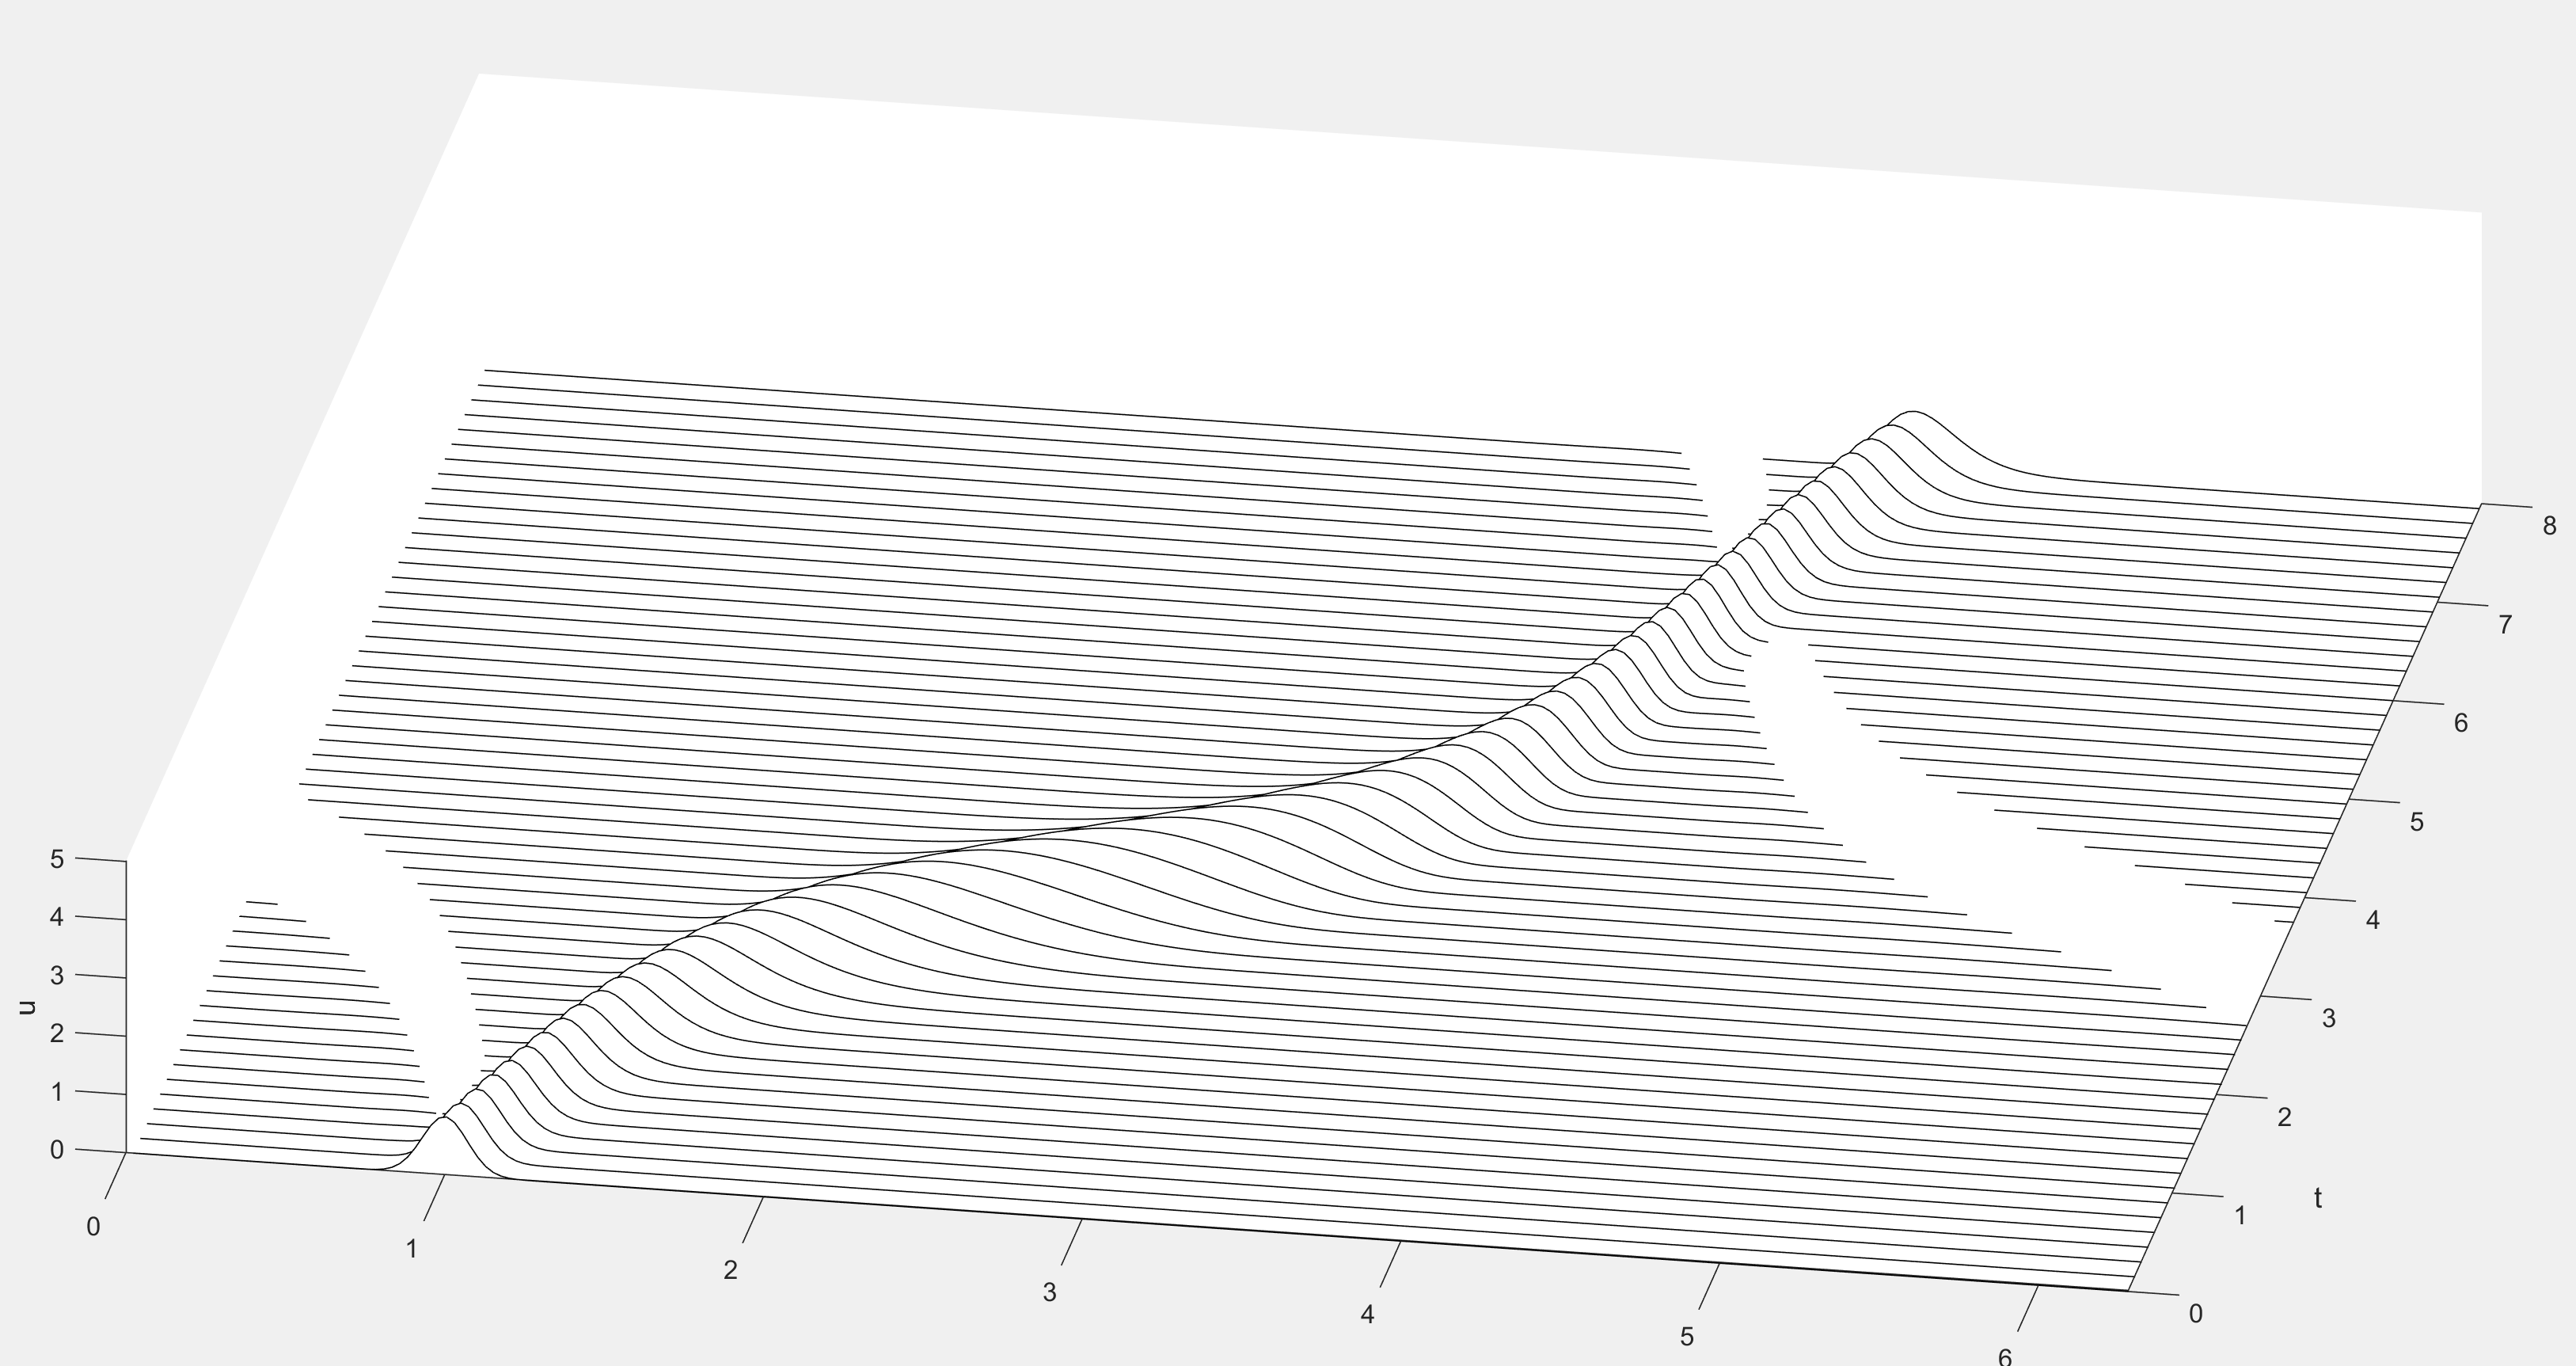
\includegraphics[scale=0.35]{3_77}
\end{center}
\textbf{•}\\
3.8 \\
Graphs produced:
\begin{center}
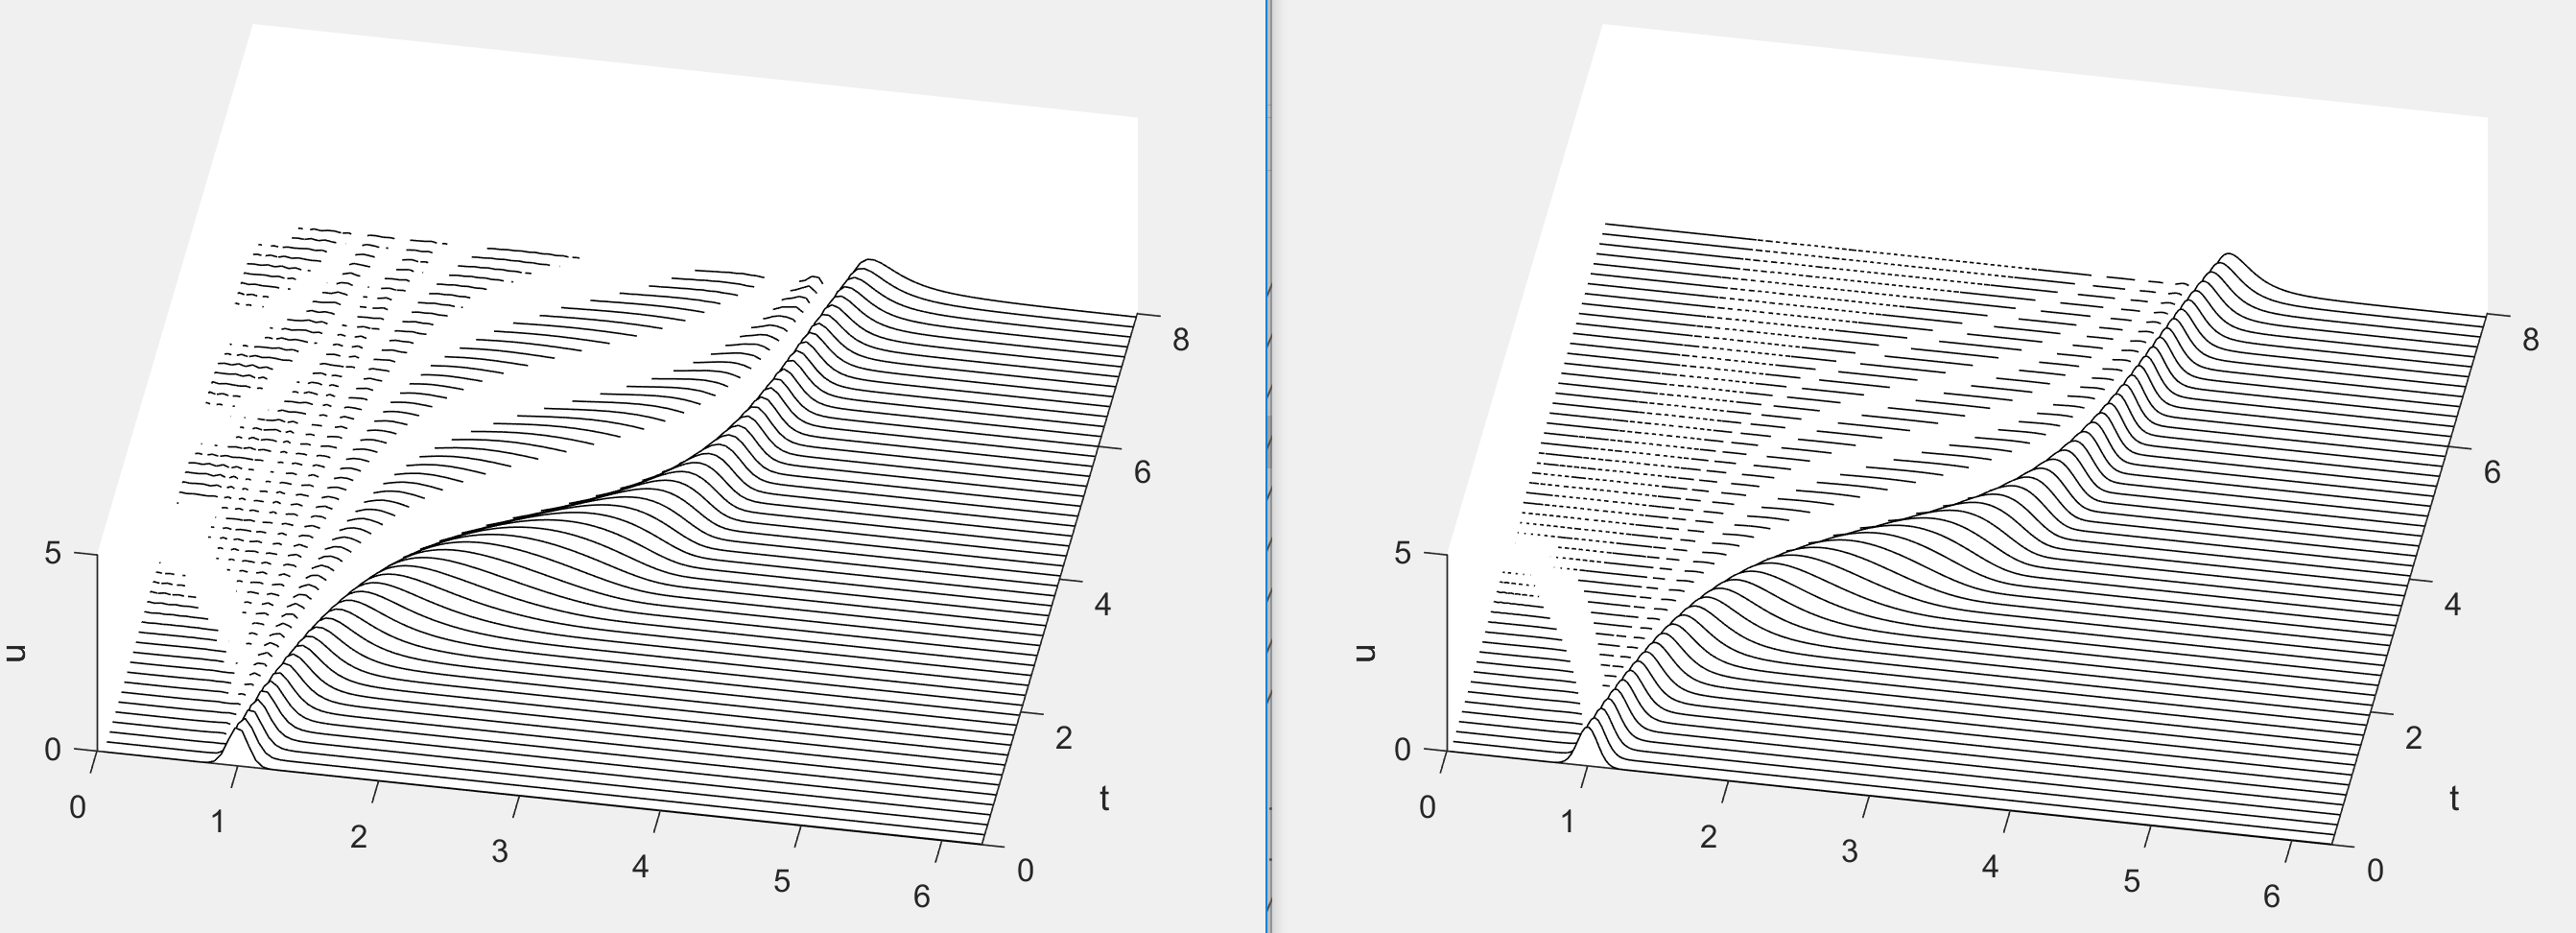
\includegraphics[scale=0.55]{3_7}
\end{center}
The difference between using the finite difference leap from formula over using the spectral one is very apparent in the graphs above as directly to the left of the curve it has a warping directly next to the curve and several more smaller warpings further to the left. Increasing N to 256 does help reduce these warping but does not produce anywhere nearly as smooth a curve as that the spectral method does.
\textbf{•}\\




\end{document}


